%***************************************************************************************************************************

\chapter{Contraste de hipótesis}
El contraste de hipótesis, o lo que se conoce como tests estadísticos, se engloba en el ámbito de la
Inferencia Estadística, que es la parte de la estadística que estudia cómo sacar conclusiones generales
(sujetas a un determinado grado de fiabilidad o significancia) para toda la población a partir del
estudio de una muestra. En nuestro caso, se tratará de sacar conclusiones de los resultados obtenidos por
diferentes algoritmos (muestra) para determinar, por ejemplo, si los algoritmos tienen un rendimiento
significativamente diferente y por lo tanto no se pueden considerar iguales (población).

El \textbf{contraste de hipótesis} es uno de los problemas más comunes dentro de la inferencia
estadística. En él se contrasta una hipótesis estadística. Por ejemplo:\\\\
\textit{Un ingeniero de software afirma que la media de los resultados obtenidos por un algoritmo
de aprendizaje automático es 10. ¿Se podría desmentir la afirmación del ingeniero?}\\\\
El planteamiento del contraste sería el siguiente  ($\mu$ indica media poblacional):
\begin{center}
$ \mu = 10 $

$ \mu \neq 10 $
\end{center}

Para tomar una decisión (desmentir o no la afirmación), hay que basarse en los datos de una muestra, para
comprobar si en efecto la media de los resultados es 10 (media muestral). Para ello, podría establecer una
regla de decisión sobre la cual se basaría nuestra decisión final. Por ejemplo: si la media obtenida está
próxima a la afirmada por el ingeniero (10), entonces se podría afirmar que dice la verdad. Si por el
contrario la muestra nos proporciona una media muy distinta a 10, entonces se puede afirmar que la evidencia
desmiente la afirmación del ingeniero sobre el algoritmo en cuestión. Esto supone un problema y es el hecho
de cuándo considerar que la media es lo suficientemente distinta como para determinar que la afirmación del
ingeniero es errónea. Por ejemplo si la media de la muestra es 8.5, ¿se podría desmentir la afirmación
inicial? El contraste de hipótesis nos proporciona una forma de establecer este criterio y poder rechazar o
aceptar la afirmación inicial.

%***************************************************************************************************************************

\section{Hipótesis nula y alternativa}
En todo contraste de hipótesis siempre se dan dos posibilidades o hipótesis, las cuales se representan con
los siguientes símbolos:
\begin{center}
$H_0:$ Hipótesis nula

$H_1:$ Hipótesis alternativa
\end{center}
\begin{itemize}
\item $H_0$: Es la hipótesis que se supone cierta de partida, es decir, es la hipótesis que establece que lo que
indica la muestra es solamente debido a la variación aleatoria entre la muestra y la población.
\item $H_1$: Es la hipótesis alternativa y es la que reemplazará a la hipótesis nula si ésta es rechazada. $H_1$
establece que lo que indica la muestra es verdadero, ya que representa a toda la población.
\end{itemize}
A modo de ejemplo, supongamos que unos programadores están trabajando en la optimización de un algoritmo
de aprendizaje. El objetivo es mejorar el algoritmo de forma que los resultados que proporcione sean menores
de 100. Se toma una muestra de los resultados obtenidos por el nuevo algoritmo optimizado y se observa que la
media de la muestra es de 92. Si no hubiera incertidumbre en la media muestral, entonces se podría concluir
que la modificación reduciría los resultados a 92. Sin embargo, siempre existe incertidumbre en la media
muestral. La media poblacional en realidad será poco mayor o menor a 92.

Los programadores están preocupados de que el nuevo algoritmo en realidad no mejore al anterior, es decir, que
la media poblacional pudiera ser mayor o igual a 100. Quieren saber si esta preocupación está justificada. Se ha
observado una muestra con media de 92 y existen dos posibles interpretaciones o, como se ha mencionado más arriba
dos tipos de hipótesis que serán contrastadas más adelante mediante un determinado test estadístico:
\begin{enumerate}
\item La media poblacional es mayor o igual a 100 (la media muestral es, por tanto, menor debido sólo a la
variación aleatoria de la media poblacional). El nuevo algoritmo no mejorará al anterior.
\item La media poblacional es menor que 100, y la media muestral lo refleja. El nuevo algoritmo sí mejorará
al anterior.
\end{enumerate}
La primera interpretación sería la hipótesis nula o $H_0$. La segunda, la hipótesis alternativa o $H_1$, como bien
se comentó más arriba.

En este caso, los programadores están preocupados de que la hipótesis nula sea cierta. Un test estadístico o
prueba de hipótesis hallará una medida cuantitativa de la factibilidad de la hipótesis nula (denominado
estadístico de contraste, que para este ejemplo viene dado por la media obtenida en la muestra) y se podrá
decir a los programadores (después de que el test tome la decisión) si su preocupación está o no justificada.
Por tanto, a modo de resumen este ejemplo nos proporciona dos hipótesis:
$$H_0: \mu \geq 100 \mbox{ vs. } H_1: \mu < 100$$

La realización de un contraste de hipótesis no consiste en decidir cuál de las dos hipótesis ($H_0$, $H_1$) es más
creíble, sino en decidir si la muestra proporciona o no suficiente evidencia para descartar $H_0$. Para realizar la
prueba de hipótesis o test estadístico se pone la hipótesis nula en juicio, es decir se empieza suponiendo que $H_0$
es verdadera. Se podría poner como analogía el supuesto de \textit{``En un juicio, el acusado siempre es inocente
hasta que se demuestre lo contrario."} Esto es:
\begin{center}
$H_0:$ El acusado es inocente

$H_1:$ El acusado es culpable
\end{center}
y, mientras no se tenga suficiente evidencia para aceptar $H_1$, hay que creer que lo que dice $H_0$ es cierto. La
muestra aleatoria proporcionará la evidencia. Si el juicio (test o prueba de hipótesis) determina que el acusado
es inocente, sólo se puede decir que no se tiene suficiente evidencia para asegurar que el acusado es culpable,
mientras que si aceptamos la hipótesis alternativa, se estará bastante seguro de que el acusado sí es culpable.

%***************************************************************************************************************************

\section{Estadístico de contraste} \label{estadistico}
Los tests estadísticos o pruebas de hipótesis, calculan internamente una medida cuantitativa que proporciona la
factibilidad de la hipótesis nula. Esta medición se extrae de la muestra proporcionada. Por ejemplo, si queremos
contrastar la hipótesis de que la media poblacional es 5, un estadístico a calcular puede ser la media de una
muestra. En este caso, la muestra viene determinada por los resultados obtenidos por los algoritmos y cada uno de
los tests tiene una forma particular de hallar este estadístico mediante una fórmula que lo caracteriza. Estos
estadísticos siguen una determinada distribución de probabilidad. Por ejemplo en este proyecto, los tests
implementados harán uso de estadísticos que siguen distribuciones como:
\begin{itemize}
\item Distribución normal (p. ej. test de Wilcoxon).
\item Distribución chi-cuadrado $\chi^2$ (p. ej. test de Friedman).
\item Distribución f de Fisher-Snedecor (p. ej. test de Iman-Davenport).
\item Distribución t de Student (p. ej. t-test).
\end{itemize}
La figura \ref{fig:pdf}, nos muestra el aspecto que presentan las distintas distribuciones de probabilidad. Las
distribuciones dependen de ciertos parámetros para determinar su forma ($\mu$, $\sigma^2$...): 
\begin{figure}[h]
\centering
\subfigure[Distribución normal con media $\mu$ y varianza $\sigma^2$.]{
\label{fig:pdfa}
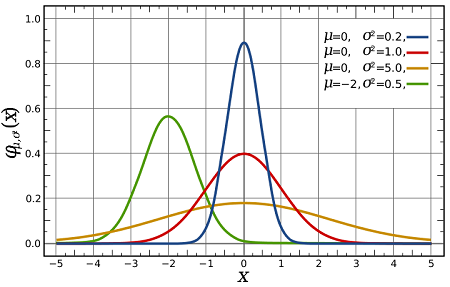
\includegraphics[width=5cm,height=3cm]{figuras/pdf_normal.png} }
\subfigure[Distribución $\chi^2$ con $K$ grados de libertad.]{
\label{fig:pdfb}
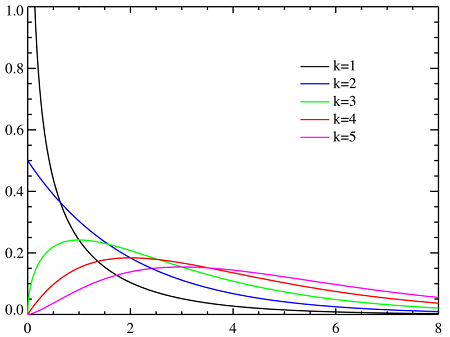
\includegraphics[width=5cm,height=3cm]{figuras/pdf_chi_cuadrado.png} }
\end{figure}
\begin{figure}[h]
\centering
\subfigure[Distribución f con $d1$ y $d2$ grados de libertad.]{
\label{fig:pdfc}
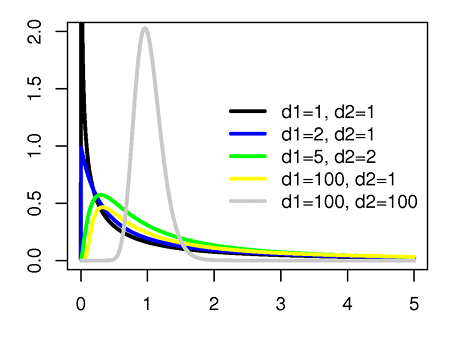
\includegraphics[width=5cm,height=3cm]{figuras/pdf_f.png} }
\subfigure[Distribución t con $K$ grados de libertad.]{
\label{fig:pdfd}
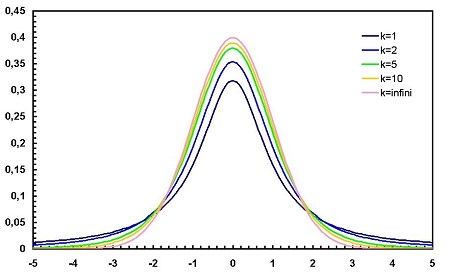
\includegraphics[width=5cm,height=3cm]{figuras/pdf_t_student.jpg} }
\caption{Distribuciones de probabilidad.}
\label{fig:pdf}
\end{figure}
\newline
Como podemos ver en la figura \ref{fig:pdf}, la distribución normal presenta $\mu$ y $\sigma^2$ como parámetros.
Éstos indican media y varianza respectivamente. La varianza, es una medida de dispersión que indica cómo se
distribuye la población. Por ejemplo: en una distribución normal de media 0 y varianza 1, que es la línea roja
en la figura \ref{fig:pdfa}, aproximadamente el $68\%$ de la población se encuentra en el intervalo $[-1,1]$,
ya que el área bajo la curva es de 0.68. Por tanto, la probabilidad de que un individuo de la población se
encuentre en ese intervalo es del 68\%. Si un estadístico sigue una distribución normal con media $\mu$ y
varianza $\sigma^2$, se expresa como:
\[ \mbox{Estadístico} \sim N(\mu,\sigma^2) \]
En las distribuciones $\chi^2$ y t de Student se habla del parámetro $K$ o grados de libertad ($d1$ y $d2$  en
la distribución f de Fisher-Snedecor). La media y la varianza de estas tres distribuciones vendrán determinadas por
el parámetro $K$. Cuando se habla de grados de libertad se está refiriendo al número de valores que se pueden elegir
libremente en una muestra. Por ejemplo: una muestra con dos datos y media 5 si el primer dato toma el valor 4 entonces
necesariamente el segundo dato debe de ser 6 (para lograr la media de 5). En este caso, se tienen:
\begin{center}
$N - 1$ grados de libertad, donde $N$ es el tamaño de la muestra.
\end{center}
Se hallan con la fórmula $N-R$, donde $N$ es el número de individuos en la muestra cuyo valor puede ser elegido de
forma libre y $R$ es el número de sujetos cuyo valor dependerá del valor que tengan los individuos de la muestra que
son libres. También se puede representar por $K-R$, donde $K$ es el número de grupos (cuando intervienen grupos y
no sujetos individuales).

En nuestro caso, $N$ viene determinado por el número de resultados obtenidos por los algoritmos (número de filas
de la matriz de la muestra de datos) y $K$ por el número de algoritmos o variables relacionadas que tiene la muestra
de datos con la que se están aplicando los tests (número de columnas de la matriz). Cada test que use el parámetro
de grados de libertad lo calcula de acuerdo a su fórmula característica para el estadístico. 

Todas las distribuciones de la figura \ref{fig:pdf} son continuas, pues se puede tomar cualquier valor dentro de un
intervalo, a diferencia de las distribuciones discretas. Por otra parte, en la distribución t de Student a medida que
aumentan los grados de libertad se tiende más a una distribución normal estandarizada (de $\mu = 0$ y $\sigma^2 = 1$).

Las distribuciones de probabilidad que puedan seguir un estadístico nos dan un valor diferente de probabilidad para
cada valor diferente del estadístico. Este valor de probabilidad indica cómo de probable que es obtener ese valor del
estadístico siendo la hipótesis nula cierta. Por ejemplo, si es cierta la hipótesis nula de que la media de una población
es 5, es más probable que obtengamos una media de una muestra igual a 4.5 que a 3.

%***************************************************************************************************************************

\section{Decisiones y tipos de error} \label{tipos_error}
Cuando se lleva a cabo un contraste de hipótesis sólo se pueden tomar dos decisiones. Los datos de la muestra,
que en este proyecto vendrá dada por los resultados obtenidos por los algoritmos, evidenciarán qué decisión se
debe tomar:
\begin{enumerate}
\item Aceptar la hipótesis nula ($H_0$) (Rechazar la hipótesis alternativa $H_1$)
\item Rechazar $H_0$ (Aceptar la hipótesis alternativa)
\end{enumerate}
Sin embargo, cuando se toma la decisión se pueden cometer dos tipos de error. La figura \ref{fig:decision}, nos
muestra las decisiones y los dos tipos de errores que se pueden cometer:
\begin{figure}[h]
\centering
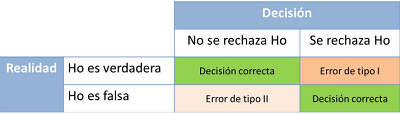
\includegraphics[width=7cm,height=2cm]{figuras/tipos_error.png}
\caption{Decisiones y tipos de error.}
\label{fig:decision}
\end{figure}
\newpage
La probabilidad de ``Error tipo I" se denota por $\alpha$ y se denomina nivel de significación:
\begin{center}
$P(\mbox{``Error tipo I}") = P(\mbox{Rechazar } H_0|H_0 \mbox{ es cierta}) =\alpha$
\end{center}
El nivel de significación consiste en la probabilidad de rechazar la hipótesis nula $H_0$ cuando verdaderamente
es cierta. Este valor $\alpha$ es un parámetro que debe seleccionar la persona que quiere realizar un test
estadístico en base a cómo de importante considere rechazar $H_0$ cuando es cierta. Normalmente es del 5\%, lo
que implicará que 5 de cada 100 veces se acepta la hipótesis alternativa cuando la cierta es la hipótesis nula.
Cuanto menor sea el nivel de significación, cada vez es más difícil rechazar la hipótesis nula. Es decir, si
queremos equivocarnos menos veces, necesitamos mucha más evidencia para justificar el rechazo. Si es grande es
más fácil aceptar la hipótesis alternativa cuando en realidad es falsa.
\\Por otra parte, la probabilidad de ``Error tipo II" se denota por $\beta$:
\begin{center}
$P(\mbox{``Error tipo II}") = P(\mbox{Aceptar } H_0|H_0 \mbox{ es falsa}) =\beta$
\end{center}
Este error $\beta$ consiste en la probabilidad de aceptar la hipótesis nula $H_0$ cuando verdaderamente es
falsa.
\\Por último, cabe destacar el concepto de ``Potencia".
\begin{center}
$P(\mbox{``Potencia}") = P(\mbox{Rechazar } H_0|H_0 \mbox{ es falsa}) =1-\beta.$
\end{center}
La potencia es la probabilidad de detectar que una hipótesis es falsa. Los tests estadísticos o pruebas de hipótesis
implementados en el presente proyecto se caracterizan por su potencia, siendo esta fija, y dejando como parámetro
libre el nivel de significación. Así, cuanto mayor es el nivel de potencia, mejor será el test, ya que se rechazarán
más hipótesis nulas cuando se deben rechazar (mayor habilidad en aceptar correctamente hipótesis alternativas).

En este proyecto se pondrá el énfasis en el nivel de significación, ya que es la hipótesis alternativa la que se
quiere probar y no se quiere aceptar si en realidad no es cierta, es decir, si aceptamos la hipótesis alternativa
queremos equivocarnos con un margen de error muy pequeño. Obviamente, lo ideal sería que tanto $\alpha$ como
$\beta$ fuesen nulos y que no se cometiese ningún error, o que ambos valores fuesen muy pequeños. Como no se pueden
disminuir ambos errores a la vez, se controla el ``Error tipo I".

%***************************************************************************************************************************

\section{Intervalos de confianza}
El nivel de significación fijado divide en dos regiones el conjunto de posibles valores del estadístico de
contraste: la región de aceptación y la región de rechazo o región crítica. Se denomina región de aceptación
a la región que conduce a la aceptación de $H_0$ y región de rechazo a la región que conduce al rechazo de $H_0$
en favor de $H_1$. Aquí surge el concepto de ``Cola", que indica la porción o porciones de una distribución
de probabilidad en la cual se rechaza la hipótesis nula, es decir, la región de rechazo.

La determinación de las regiones de aceptación o de rechazo depende de cómo se establezca la hipótesis
alternativa $H_1$. Por ejemplo, si hablamos de un contraste en el que se esté contrastando una determinada
media ($\mu_0$) se podría establecer como $H_1$ que la media en realidad sea menor, mayor o distinta a
($\mu_0$):\\\\
\begin{itemize}
\item Media menor (test unilateral con cola a la izquierda):
\end{itemize}
\begin{center}
$H_0: \mu = \mu_0$
\\$H_1: \mu < \mu_0$
\end{center}
\begin{itemize}
\item Media mayor (test unilateral con cola a la derecha):
\end{itemize}
\begin{center}
$H_0: \mu = \mu_0$
\\$H_1: \mu > \mu_0$
\end{center}
\begin{itemize}
\item Media distinta (test bilateral o de dos colas):
\end{itemize}
\begin{center}
$H_0: \mu = \mu_0$
\\$H_1: \mu \neq \mu_0$
\end{center}
En la figura \ref{fig:intervalos_normal}, podemos ver cómo quedarían establecidos los intervalos para el ejemplo. En
rojo se muestra la región de rechazo:
\begin{figure}[h]
\centering
\subfigure[Test unilateral. Cola a la izquierda.]{
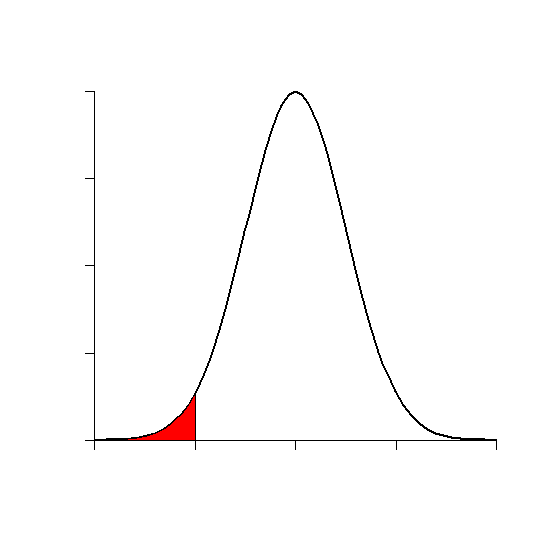
\includegraphics[width=5cm,height=3cm]{figuras/test_unilateral_izq.png} }
\subfigure[Test unilateral. Cola a la derecha.]{
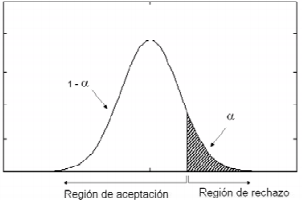
\includegraphics[width=5cm,height=3cm]{figuras/test_unilateral_der.png} }
\end{figure}
\begin{figure}[h]
\centering
\subfigure[Test bilateral o de dos colas.]{
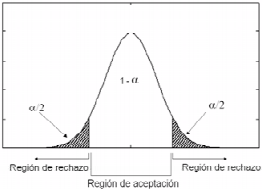
\includegraphics[width=5cm,height=3cm]{figuras/test_bilateral.png} }
\caption{Regiones de aceptación y rechazo.}
\label{fig:intervalos_normal}
\end{figure}

Como se puede observar en el caso del test bilateral o de dos colas, el $\alpha$ se divide en dos porciones iguales:
$\alpha / 2$, que constituye la región de rechazo. La región de aceptación tendrá en todos los casos probabilidad
$1 - \alpha$.

%***************************************************************************************************************************

\section{Decisión final y Concepto de $p-valor$}
Si el valor del estadístico cae en la región de aceptación, se acepta la hipótesis nula, ya que no existen
razones suficientes para rechazar $H_0$ con el nivel de significación dado. Por tanto, en este caso se diría
que el contraste es estadísticamente no significativo, es decir, no existe evidencia estadísticamente significativa
en favor de $H_1$.
\begin{figure}[h]
\centering
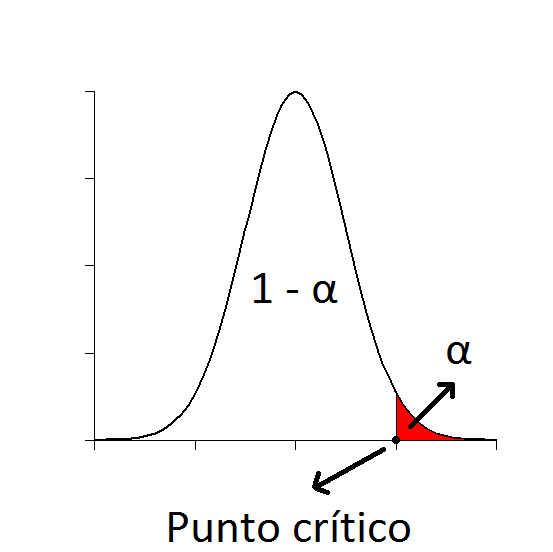
\includegraphics[width=5cm,height=3cm]{figuras/critico.png}
\caption{Punto crítico.}
\label{fig:punto_critico}
\end{figure}
La figura \ref{fig:punto_critico} nos muestra el punto crítico: si el estadístico obtenido por el test o
prueba de hipótesis es 5 y el punto crítico es 4.5, se rechaza $H_0$ ya que el estadístico pertenece a la
región de rechazo.

La decisión de rechazar o aceptar la hipótesis nula, se puede determinar también mediante el $p-valor$,
que es el parámetro utilizado para realizar los tests estadísticos en este proyecto. El $p-valor$ proporciona
un forma más eficiente de determinar si el contraste es o no estadísticamente significativo, ya que no sería
necesario recalcular regiones de aceptación y rechazo cada vez que el usuario de los tests cambia de nivel de
significación.

\begin{center}
``El $p-valor$, es la probabilidad que hay de obtener un valor al menos tan extremo como el estadístico en cuestión
que se ha obtenido."
\end{center}

Para entender mejor el concepto de $p-valor$, conviene hablar de las distribuciones de probabilidad vistas en la
figura \ref{fig:pdf} de la sección \ref{estadistico} donde se hablaba del estadístico de contraste. Estas
distribuciones son funciones que se denominan ``Funciones de densidad de probabilidad" (FDP). Como bien se
expuso, estas funciones proporcionan la probabilidad que existe para cada valor diferente del estadístico (cómo
de probable es obtener ese valor del estadístico). Si en vez de trabajar con las funciones de densidad de 
probabilidad, se trabaja con las funciones de distribución acumuladas (FDA), para cada valor del estadístico
éstas devolverían la probabilidad de obtener un valor igual o menor que ese estadístico siendo la hipótesis nula
cierta. En la figura \ref{fig:comparativa_pdf_cdf} podemos ver una comparación entre los dos tipos de funciones
para el caso de la distribución $\chi^2$:

\begin{figure}[h]
\centering
\subfigure[Función de densidad de probabilidad.]{
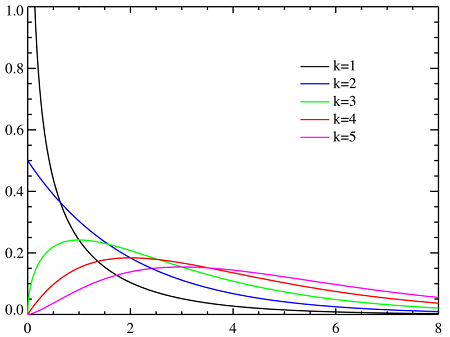
\includegraphics[width=5cm,height=3cm]{figuras/pdf_chi_cuadrado.png} }
\subfigure[Función de distribución acumulada.]{
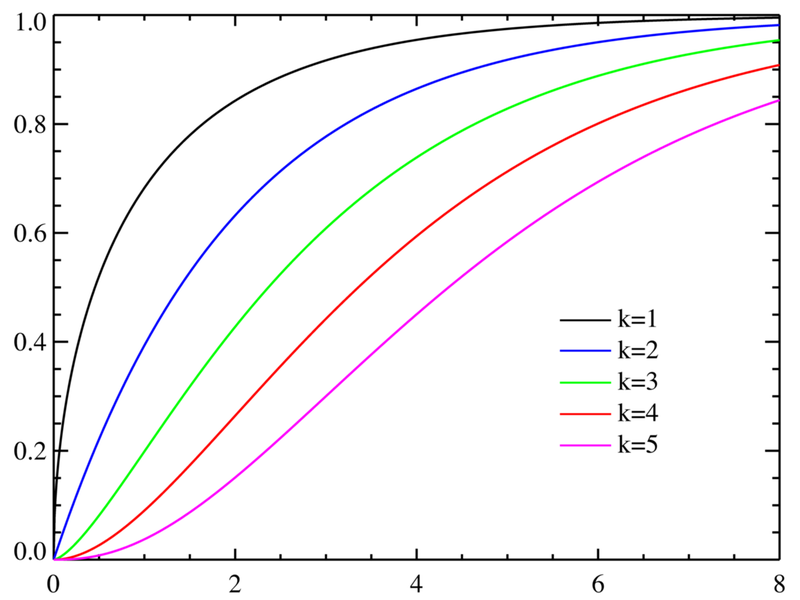
\includegraphics[width=5cm,height=3cm]{figuras/cdf_chi_cuadrado.png} }
\caption{Comparativa FDP y FDA.}
\label{fig:comparativa_pdf_cdf}
\end{figure}

Visto de otro modo, con la distribución acumulada, dado un estadístico, nos devuelve la probabilidad que hay de
obtener un valor al menos tan extremo como el estadístico en cuestión. Esto es el $p-valor$. Por ejemplo si el valor
del estadístico es 3 y el test da como resultado un $p-valor$ igual a 0.1, esto quiere decir que un 10\% de las veces
vamos a obtener un valor similar. Si el $p-valor$ es muy bajo, es decir, la probabilidad de obtener un valor al menos
tan extremo como ese estadístico es muy baja, se puede concluir que la hipótesis nula no es cierta, ya que sería
poco probable que siendo cierta se obtuviese ese estadístico.

El criterio para saber si el $p-valor$ es lo suficientemente bajo como para rechazar que la hipótesis nula sea cierta
es tomado de acuerdo al nivel de significancia establecido. Como se ha mencionado en la sección \ref{tipos_error}, el
nivel de significancia o $\alpha$ indica la probabilidad de rechazar la hipótesis nula siendo ésta cierta. Si el
$p-valor$ es menor que el nivel de significancia se rechaza la hipótesis nula.

Según se disminuye $\alpha$, cada vez es más difícil de rechazar la hipótesis nula, ya que se necesita mucha más
evidencia para justificar el rechazo. Por ejemplo si $\alpha$ es 0.05 y la probabilidad de obtener un estadístico
igual a 1 es 0.03, se rechaza la hipótesis nula. Sin embargo, si el $\alpha$ fuese 0.01, no se podría rechazar: no hay suficiente evidencia de que la hipótesis nula sea falsa.

%***************************************************************************************************************************

\section{Etapas en la resolución de un contraste de hipótesis}
En un contraste de hipótesis siempre se siguen una serie de pasos definidos. Como se ha ido viendo a lo largo
del capítulo, los pasos para la realización de una prueba de hipótesis o test estadístico son las siguientes
\cite{libro}:
\begin{enumerate}
\item Especificación de la hipótesis nula $H_0$ y de la hipótesis alternativa $H_1$.
\item Suponer que $H_0$ es verdadera (el test sirve para que a partir de la muestra de datos podamos rechazar
$H_0$ en beneficio de $H_1$).
\item Calcular un estadístico de prueba o estadístico de contraste. Este estadístico se usa para evaluar la
fuerza de la evidencia en contra de $H_0$ (medir la discrepancia entre la hipótesis y la muestra).
\item Establecer un nivel de significación $\alpha$ en base a cómo de importante se considere rechazar $H_0$
cuando realmente es verdadera.
\item El nivel de significación fijado divide en dos regiones el conjunto de posibles valores del estadístico
de contraste: la región de aceptación y la región de rechazo o región crítica.
\item Si el valor del estadístico cae en la región de rechazo, se rechaza la hipótesis nula, ya que esto
evidencia que los datos obtenidos de la muestra no son compatibles con $H_0$. Por tanto, en este caso se diría
que el contraste es estadísticamente significativo, es decir, existe evidencia estadísticamente significativa en
favor de $H_1$.
\item Si el valor del estadístico cae en la región de aceptación, se acepta la hipótesis nula, ya que no existen
razones suficientes para rechazar $H_0$ con el nivel de significación dado. Por tanto, en este caso se diría
que el contraste es estadísticamente no significativo, es decir, no existe evidencia estadísticamente significativa
en favor de $H_1$.
\item La decisión de rechazar o aceptar la hipótesis nula, se puede determinar también mediante el $p-valor$,
que es el parámetro utilizado para realizar los tests estadísticos en este proyecto. El $p-valor$ proporciona
un forma más eficiente de determinar si el contraste es o no estadísticamente significativo, ya que no sería
necesario recalcular regiones de aceptación y rechazo cada vez que el usuario de los tests cambia de nivel de
significación.
\end{enumerate}

%***************************************************************************************************************************

\section{Tests paramétricos}
Uno de los tipos más comunes de tests son los tests paramétricos. En general, estos tests son más robustos y
tienen mayor potencia que los tests no paramétricos, que se verán más adelante en \ref{no_parametricos}. Sin
embargo, las pruebas paramétricas se basan en supuestos que muy probablemente se violan cuando se analiza el
rendimiento de algoritmos de inteligencia computacional y minería de datos \cite{parametricos}. Estas suposiciones
o condiciones paramétricas que deben cumplir los resultados de los algoritmos son explicadas a continuación.

%----------------------------------

\subsection{Condiciones Paramétricas}

\subsubsection{Independencia}
En estadística, dos eventos son independientes si cuando uno de ellos se da no modifica la probabilidad de la
ocurrencia del otro. Dicho de otra forma: cuando las muestras o datos obtenidos por los algoritmos, es decir, los
resultados de éstos no dependen unos de otros. Cuando se comparan dos algoritmos de optimización normalmente suelen
ser independientes. Cuando se comparan dos métodos de aprendizaje automático, depende de cómo sea la partición.
La independencia es una característica que en este proyecto debe asumir el usuario de los tests, y, por tanto,
podrá actuar de una forma u otra bajo su responsabilidad.

\subsubsection{Normalidad}
Una muestra u observación es normal cuando su comportamiento sigue una distribución normal (o distribución de
Gauss) con una cierta media $\mu$ y varianza $\sigma^2$. En la figura \ref{fig:normalidad} podemos ver que a la
izquierda se cumple el supuesto de normalidad, mientras que a la derecha los datos de la muestra no están distribuidos
de forma normal:

\begin{figure}[h]
\centering
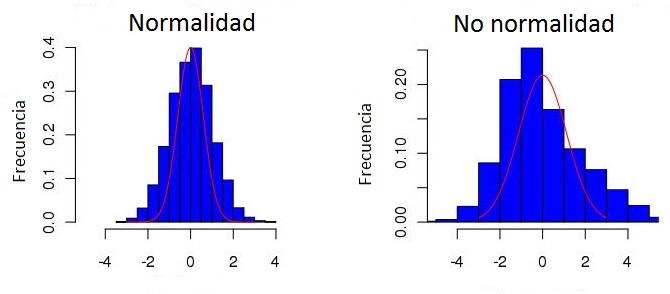
\includegraphics[width=9cm,height=3cm]{figuras/normalidad.jpg}
\caption{Normalidad VS No normalidad.}
\label{fig:normalidad}
\end{figure}

En este proyecto se pueden realizar los siguientes tests no paramétricos para comprobar el supuesto de normalidad:

\begin{itemize}
\item \textbf{Shapiro–Wilk:} Contrasta la hipótesis nula de que las muestras o poblaciones provienen de una
población normalmente distribuida. Analiza la muestra para hallar el nivel de simetría y Kurtosis (forma de
la curva) para calcular la diferencia con respecto a una distribución normal, obteniendo el p-valor de la suma
de los cuadrados de estas discrepancias. Se considera de los más potentes, sobre todo para muestras de menos
de 30 elementos. Sin embargo, el rendimiento de esta prueba se ve afectado de forma negativa cuando no existe
independencia en los datos.
\item \textbf{D’Agostino–Pearson:} Contrasta la hipótesis nula de que las muestras o poblaciones provienen de
una población normalmente distribuida. Primero calcula el coeficiente de asimetría (en qué medida la normal es
simétrica ó coeficiente 0) y el coeficiente de Kurtosis (grado de amplitud, donde lo normal es coeficiente 0) para
cuantificar qué tan lejos se está de la distribución normal. Luego, calcula cómo de lejos cada uno de estos valores
difiere de los valores esperados en una distribución normal, para obtener el $p-valor$ de la suma de estas
discrepancias. Es menos potente que el test de Shapiro-Wilk, pero no se ve afectado cuando los datos no son
independientes.
\item \textbf{Kolmogorov–Smirnov:} Realiza una prueba de bondad de ajuste, para determinar si los datos observados
de la muestra se ajustan a la distribución normal. Tiene como $H_0$ que la distribución obtenida de los datos
observados es idéntica a la distribución normal. Es la prueba que menos potencia presenta de los tres y, por tanto
es la que peor funciona.
\end{itemize}

\subsubsection{Homocedasticidad}
La homocedasticidad es la condición que dice que las poblaciones de entrada o datos obtenidos por los algoritmos
proceden de poblaciones con varianzas iguales. Es decir, esta propiedad indica la hipótesis de igualdad de
varianzas. El caso contrario sería heterocedasticidad. En la figura \ref{fig:homocedasticidad} se puede apreciar
la diferencia existente entre unos datos que proceden de poblaciones con varianzas similares y aquellos que
no:

\begin{figure}[h]
\centering
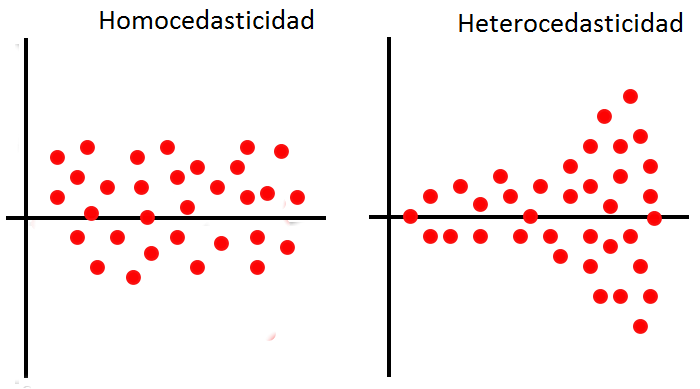
\includegraphics[width=6cm,height=3cm]{figuras/homocedasticidad.png}
\caption{Homocedasticidad VS Heterocedasticidad.}
\label{fig:homocedasticidad}
\end{figure} 

En este proyecto se puede realizar el siguiente test no paramétrico para comprobar el supuesto de homocedasticidad:

\begin{itemize}
\item \textbf{Test de Levene:} Contrasta la hipótesis nula de que todas las poblaciones de entrada proceden de
poblaciones con varianzas iguales. Se utiliza para comprobar si K muestras pertenecientes a datos obtenidos por
K algoritmos presentan o no homogeneidad de varianzas. 
\end{itemize}

%----------------------------------

\subsection{Test Anova}
El análisis de la varianza (ANOVA) es uno de los tests estadísticos más ampliamente utilizados para probar
la igualdad de más de dos medias de la población. Se trata de una versión más general del T-test, ya que permite
comparar más de 2 poblaciones (en este proyecto resultados de más de dos algoritmos). Dado que es un test
paramétrico, se asume que se dan las condiciones de independencia, normalidad y homocedasticidad en su
aplicación. De no ser el caso, los resultados de esta prueba no son fiables.

\subsubsection{Hipótesis}
\begin{itemize}
\item Hipótesis nula $H_0$: $\mu_1 = \mu_2 = \mu_3 ... = \mu_K$.
\item Hipótesis alternativa $H_1$: $\exists \quad \mu_j \neq \mu \quad j=1,2,...,K$.
\end{itemize}
La hipótesis nula indica que las medias de distintas poblaciones o muestras coinciden $(K>2)$, frente a la
hipótesis alternativa de que por lo menos una de las poblaciones tiene una media que difiere de las demás. Es,
por tanto, un contraste o prueba unilateral con cola a la derecha. En este proyecto el parámetro $K$ viene
determinado por el número de algoritmos que existe en la muestra de datos.

\subsubsection{Pasos a desarrollar}
Los pasos a seguir para realizar el test de Anova son los siguientes:
\begin{itemize}
\item Se analiza la variación total (respecto a la media general o media de medias de los resultados de cada
algoritmo):
\[ variacion\_t = \sum_{i=1}^{N} \sum_{j=1}^{K} (X_{ij} - \bar{X})^2 \]
, donde $\bar{X}$ es la media general, $N$ es el número de conjuntos de datos o problemas sobre los que se
aplican los algoritmos y $X_{ij}$ es un resultado específico obtenido por un algoritmo.
\item Se halla también la variación entre los diferentes tratamientos o algoritmos (efecto de la media de cada
tratamiento respecto a la media general):
\[ variacion\_tr = \sum_{i=1}^{K} N (\bar{X}_i - \bar{X})^2 \]
, donde $\bar{X}_i$ representa la media del tratamiento o algoritmo.
\item La variación dentro del tratamiento o variación del error (cada valor respecto a la media de su tratamiento):
\[ variacion\_e = \sum_{i=1}^{N} \sum_{j=1}^{K} (X_{ij} - \bar{X}_{j})^2 \]
, donde $\bar{X}_{j}$ representa la media de un tratamiento o algoritmo.
\item Se calculan los grados de libertad totales, del tratamiento y del error como:
\[ GLT = (NK)-1 \]
\[ GLTR = K-1 \]
\[ GLE = GLT - GLTR \]
\item Luego, se determinan los cuadrados medios totales ($CMT$), del tratamiento ($CMTR$) y del error ($CME$),
que son las variaciones divididas entre los grados de libertad correspondientes.
\item Se halla el estadístico, que se distribuye como una distribución f con $K-1$ y $(KN)-K$ grados de libertad:
\[ anova = CMT / CME \]
\item Por último se halla el $p-valor$ y se toma la decisión en función del nivel de significancia.
\end{itemize}

%----------------------------------

\subsection{T-test}
El caso más simple de Anova donde intervienen únicamente 2 muestras o algoritmos es realizado por este test.
Dado que es un test paramétrico, se asume que se dan las condiciones de independencia, normalidad y homocedasticidad
en su aplicación. De no ser el caso, los resultados de esta prueba no son fiables.

\subsubsection{Hipótesis}
\begin{itemize}
\item Hipótesis nula $H_0$: $\mu_1 = \mu_2$.
\item Hipótesis alternativa $H_1$: $\mu_1 \neq \mu_2$.
\end{itemize}
La hipótesis nula indica que las medias de las 2 poblaciones o muestras coinciden, frente a la hipótesis alternativa
de que son distintas. Se trata, por tanto, de un contraste o prueba bilateral.

El estadístico de este test, se distribuye como una distribución t de Student con $N-1$ grados de libertad.

%----------------------------------

%***************************************************************************************************************************

\section{Tests no paramétricos} \label{no_parametricos}
Cuando los datos obtenidos de la aplicación de los algoritmos de aprendizaje automático no cumplen las
características de independencia, normalidad u homocedasticidad total o parcialmente podemos hablar de tests
no paramétricos. Recientemente, los tests estadísticos no paramétricos han emergido como una metodología
eficaz, robusta y asequible para la evaluación de nuevas propuestas de metaheurísticas y algoritmos evolutivos,
alcanzando gran popularidad. La validación de nuevos algoritmos requiere con frecuencia la definición
de un marco experimental exhaustivo y la parte crítica de estas comparaciones recae en la validación
estadística de los resultados, contrastando las diferencias encontradas entre métodos. Dentro de las técnicas
disponibles, destacan los tests no paramétricos debido a su flexibilidad y a las pocas restricciones de
uso que presentan (a diferencia de los tests paramétricos, los cuales sufren a menudo problemas derivados
de la imposibilidad de cumplir las condiciones paramétricas para su uso). \cite{no_parametricos}

%----------------------------------

\subsection{Test de Wilcoxon}
La prueba de los rangos con signo de Wilcoxon también conocida como el test de Wilcoxon es una prueba no
paramétrica que se utiliza como alternativa a la prueba t de Student cuando no se puede suponer la normalidad
de las muestras. Es, por tanto, menos potente que que la prueba t de Student. El test de Wilcoxon fue creado
por Frank Wilcoxon y publicado en 1945 \cite{wilcoxon}.

Sirve para comparar dos métodos o tratamientos (en este proyecto interesa comparar dos algoritmos). Por tanto,
los individuos (los problemas) donde se aplican los algoritmos tienen que ser los mismos. Es decir, a un mismo
individuo se le efectúa la medición de dos variables: las muestras son apareadas. Para tomar la decisión, hay
que basarse en las observaciones de N individuos independientes (sin relación existente entre ellos). Para tamaños
muestrales pequeños, se puede determinar mediante la comparación del estadístico con el valor crítico de la
tabla de Wilcoxon. Para tamaños muestrales grandes ($> 25$), el test se puede aproximar con la distribución normal.

\subsubsection{Hipótesis}
\begin{itemize}
\item Hipótesis nula $H_0$: $Mediana_{diferencias} = 0$.
\item Hipótesis alternativa $H_1$: $Mediana_{diferencias} \neq 0$.
\end{itemize}
La mediana, es el valor que ocupa el lugar central de todos los datos cuando éstos están ordenados de menor a
mayor. $H_0$ indica que la mediana de las diferencias de dos muestras (resultados de dos algoritmos) relacionadas
son iguales, es decir, las dos medianas son iguales (los resultados de los algoritmos no dependen del algoritmo).
$H_1$ indica, por otra parte, que las medianas son diferentes. Se trata, por tanto, de una prueba bilateral.

\subsubsection{Pasos a desarrollar}
Los pasos a seguir para realizar la prueba de los rangos signados de Wilcoxon son los siguientes:
\begin{itemize}
\item Se calculan las diferencias entre las muestras. Por ejemplo: diferencias entre los resultados del algoritmo
A y B.
\subitem - Se eliminan los elementos que tengan diferencias nulas (se excluye el 0).
\item Se ordenan las diferencias en valor absoluto (independientemente del signo).
\item Se asignan rangos de orden 1,2,...,N. Si hay empates se calcula la media del rango de cada uno de los elementos
repetidos.
\item Suma de los rangos según los signos que tengan las diferencias para obtener los estimadores:
\subitem - $T(+) = $ Suma de los rangos correspondientes a diferencias positivas. 
\subitem - $T(-) = $ Suma de los rangos correspondientes a diferencias negativas.
\item Definir el estadístico:
\subitem - $T = \min [T(+), T(-)]$
\item Si $N \leq 25$, se examina la tabla de Wilcoxon que nos da los valores críticos (el intervalo de aceptación)
para cada valor de N y cada nivel de significancia. El contraste será estadísticamente significativo si: 
$T <= $ límite inferior correspondiente.
\item Si $N > 25$, el estadístico se ajusta a la distribución normal. Por tanto, se calcula el estadístico $Z$ y
se toma la decisión en función del $p-valor$ y del nivel de significancia:
\[ Z = \frac{T-\frac{N(N+1)}{4}}{\sqrt{\frac{N(N+1)(2N+1)}{24}}} \]
\end{itemize}

%----------------------------------

\subsection{Test de Friedman}
El test de Friedman es una prueba no paramétrica que puede realizar comparaciones entre dos o más algoritmos, es
decir, se trata de una prueba de comparaciones múltiples. Fue desarrollada por el economista Milton Friedman y
trabaja asignando rankings para establecer quién es el mejor algoritmo de la muestra de datos proporcionada.

\subsubsection{Hipótesis}
\begin{itemize}
\item Hipótesis nula $H_0$: No existen diferencias entre los algoritmos.
\item Hipótesis alternativa $H_1$: Existen diferencias entre los algoritmos.
\end{itemize}
La hipótesis nula quiere decir que todos los algoritmos se comportan de la misma forma, por lo que los rankings
que poseen deben de ser similares. La hipótesis alternativa, por el contrario, afirma que existen diferencias,
lo cual quiere decir al menos el rendimiento de un algoritmo es diferente al rendimiento que presentan los demás.
Se trata, por tanto, de un contraste o prueba unilateral con cola a la derecha.

\subsubsection{Pasos a desarrollar}
Los pasos a seguir para realizar el test de Friedman son los siguientes:
\begin{itemize}
\item En primer lugar se asignan rankings $r_{ij}$ a los resultados obtenidos por cada algoritmo $j$ en cada
problema $i$. Es decir, para cada problema o conjunto de datos se asigna un ranking cuyos valores están
comprendidos entre $1$ y $K$, donde $K$ representa el número de algoritmos que se están comparando. Los rankings
se asignan de forma ascendente (1 al mejor resultado, 2 al segundo mejor, etc.) y se tiene en cuenta la función
objetivo de los algoritmos, es decir, si lo que se pretende es minimizar o maximizar resultados.
\item En caso de que haya empates en la asignación de rankings anterior, se asignan rankings medios:
\[ r_{ij} = \frac{rep + (2pos) + 1}{2} \]
, donde $rep$ representa el número de veces que se repite el dato y $pos$ representa la posición que ocupa
el dato repetido.
\item Luego, se calculan los rankings medios de cada algoritmo en los $N$ problemas:
\[ R_j = \frac{\sum_{i=1}^{N} r_{ij}}{N} \]
\item El estadístico de Friedman se distribuye de acuerdo a una distribución $\chi^2$ con $K-1$ grados de
libertad:
\[ friedman = \frac{12N}{K(K+1)} \left[\sum R_j^2 - \frac{K(K+1)^2}{4} \right] \]
\item Por último se halla el $p-valor$ y se toma la decisión en función del nivel de significancia.
\end{itemize}

%----------------------------------

\subsection{Test de Iman-Davenport}
El estadístico de Friedman fue mejorado por Iman y Davenport, que demostraron que tenía un comportamiento
demasiado conservativo (se tiende a aceptar la hipótesis nula y, por tanto, la potencia del test es menor).

\subsubsection{Hipótesis}
\begin{itemize}
\item Similar al test de Friedman.
\end{itemize}

\subsubsection{Pasos a desarrollar}
\begin{itemize}
\item El test de Iman-Davenport hace las mismas operaciones que el test de Friedman pero en él se calcula
un estadístico más ajustado (en el que también interviene el estadístico de Friedman). Este nuevo estadístico,
se distribuye de acuerdo a una distribución f con $(K-1)$ y $(K-1)*(N-1)$ grados de libertad, donde $N$
representa el número de problemas o conjuntos de datos y $K$ el número de algoritmos:
\[ iman_d = \frac{(N-1)friedman}{N(K-1)-friedman} \]
\end{itemize}

%----------------------------------

\subsection{Test de los Rangos Alineados de Friedman}
El test de los rangos alineados de Friedman realiza comparaciones y asigna rankings teniendo en cuenta a
todos los conjuntos de datos, a diferencia del test de Friedman, que asigna rankings dentro de cada conjunto
(es decir, dentro de los resultados obtenidos por los algoritmos para cada problema en particular). Por tanto,
en este caso los valores de los rankings irán desde $1$ hasta $K*N$. Suele emplearse cuando el número de
algoritmos en la comparación es pequeño y cuando se quiera realizar una comparación entre conjuntos de datos.

\subsubsection{Hipótesis}
\begin{itemize}
\item Similar al test de Friedman.
\end{itemize}

\subsubsection{Pasos a desarrollar}
\begin{itemize}
\item Cálculo de las observaciones alineadas: primero se halla el valor de localización, que es el rendimiento
medio alcanzado por los algoritmos en cada conjunto de datos y luego se calculan las diferencias entre el
rendimiento obtenido por cada algoritmo con respecto al valor de localización dentro de un mismo conjunto de
datos.
\item Se repite el primer paso para los $N$ conjuntos de datos.
\item Se juntan todas las observaciones alineadas y se ordenan para asignar los rankings alineados desde $1$
hasta $K*N$. En caso de empates se procede asignando valores medios igual que en el test de Friedman.
\item Se calculan los rankings medios de cada algoritmo en los $N$ problemas.
\item El estadístico para esta prueba se distribuye de acuerdo a una distribución $\chi^2$ con $K-1$ grados de
libertad:
\[ rangos\_al = \frac{(K-1) \left[ \sum_{j=1}^{K} \hat{R_{j}^{2}} - (\frac{KN^2}{4})(KN+1)^2 \right]}
{\left[\frac{KN(KN+1)(2KN+1)}{6}\right] - (\frac{1}{K}) \sum_{i=1}^{N} \hat{R_{i}^{2}}} \]
, donde $\hat{R_{i}}$ y $\hat{R_{j}}$ son la suma total de los rankings del problema $i$ y del algoritmo $j$
respectivamente.
\item Por último se halla el $p-valor$ y se toma la decisión en función del nivel de significancia.
\end{itemize}

%----------------------------------

\subsection{Test de Quade}
El test de Quade considera, a diferencia del test de Friedman que considera que todos los problemas son
iguales en importancia, que algunos problemas son más difíciles o que los resultados que obtienen los algoritmos
sobre ellos son más distantes (se realiza una ponderación).

\subsubsection{Hipótesis}
\begin{itemize}
\item Similar al test de Friedman.
\end{itemize}

\subsubsection{Pasos a desarrollar}
\begin{itemize}
\item Se obtienen los rankings de cada conjunto de datos de la misma forma que en Friedman.
\item Asignación de rankings a los problemas en función del tamaño del rango de la muestra en cada
uno (diferencia entre el valor observado más alto y el más bajo). Este ranking de $1$ a $N$ usa también
rankings medios en caso de empate.
\item A partir de estos datos se pueden obtener los rankings medios finales para cada algoritmo y obtener
el estadístico, que se distribuye como una distribución f con $(K-1)$ y $(K-1)*(N-1)$ grados de libertad.
\item Por último se halla el $p-valor$ y se toma la decisión en función del nivel de significancia.
\end{itemize}

%----------------------------------

\subsection{Tests POST-HOC}
Los tests no paramétricos de ranking (test de Friedman, Iman-Davenport, Rangos Alineados de Friedman y Quade),
dan como resultado la existencia o no de diferencias significativas entre los algoritmos sobre los que se han
aplicado. Es decir, nos dice si el contraste de hipótesis es o no estadísticamente significativo. Si se rechaza
la hipótesis nula de ``todos los algoritmos son iguales", sabremos que entre los algoritmos existen diferencias.
Sin embargo, puede ocurrir que un algoritmo presente un rendimiento similar a otro u otros y por tanto se pueda
considerar igual.

Estos tests comparan los algoritmos y realizan contrastes de hipótesis entre ellos para determinar diferencias.

\subsubsection{Hipótesis}
\begin{itemize}
\item Hipótesis nula $H_0$: El algoritmo $i$ y $j$ son iguales.
\item Hipótesis alternativa $H_1$: El algoritmo $i$ y $j$ son distintos.
\end{itemize}
Se trata, por tanto, de tests que realizan contrastes bilaterales, ya que están destinados a encontrar diferencias
a posteriori en caso de que el test de ranking sea estadísticamente significativo. Se distinguen dos tipos de
comparación:

\begin{itemize}
\item Método de control: Se compara el primer algoritmo del ranking devuelto por el test de ranking con el resto
de algoritmos y por tanto habrá $K-1$ comparaciones o contrastes.
\item Comparación múltiple: Compara todos los algoritmos entre sí. El número de comparaciones o contrastes por
tanto es:
\[ m = \frac{K(K-1)}{2} \]
\end{itemize}

Todos los tests POST-HOC aproximan los valores Z (estadísticos) de una distribución normal a partir de las
diferencias entre dos rankings. La forma de aproximar estos valores $Z$ varía en función del test de ranking de
donde se provenga:

\begin{itemize}
\item Test de Friedman / Iman-Davenport:
\[ Z = \frac{(R_i - R_j)}{\sqrt{\frac{K(K+1)}{6N}}} \]
, donde $R_i$ y $R_j$ son los rankings medios obtenidos por el algoritmo $i$ y $j$ respectivamente en el test
de Friedman.
\item Test de los Rangos Alineados de Friedman:
\[ Z = \frac{\hat{R_{i}} - \hat{R_{j}}}{\sqrt{\frac{K(K+1)}{6N}}} \]
, donde $\hat{R_{i}}$ y $\hat{R_{j}}$ son los rankings medios obtenidos por el algoritmo $i$ y $j$ respectivamente en el test
de los Rangos Alineados de Friedman.
\item Test de Quade:
\[ Z = \frac {T_i - T_j}{\sqrt{\frac{K(K+1)(2N+1)(K-1)}{18N(N+1)}}} \]
, donde $T_i$ y $T_j$ son los rankings medios obtenidos por el algoritmo $i$ y $j$ respectivamente en el test
de Quade.
\end{itemize}

Luego, calculan los $p-valores$ y ordenan todos los datos en función de éstos de mayor a menor significancia (de
menor a mayor). El contraste de las hipótesis (los resultados), así como el cálculo del valor $\alpha$ y los
$p-valores$ ajustados varían en función del test aplicado. Los $p-valores$ ajustados son $p-valores$ que dependen
de toda la familia de comparaciones y no sólo de una comparación, es decir, consideran la familia de hipótesis
completa para cada pareja de algoritmos y se pueden comparar con el nivel de significancia proporcionado sin
ajustar.

\subsubsection{Tests}
\begin{itemize}
\item \textbf{Test de Bonferroni-Dunn:} El contraste de las hipótesis se realiza comparando cada $p-valor$ con
el nivel de significancia ajustado:
\[ alpha\_ajustado = \frac{\alpha}{(K-1)} \]
\item \textbf{Test de Holm:} Compara cada $p-valor$ (empezando por el más significativo) con:
\[ alpha\_ajustado_i = \frac{\alpha}{(K-i)} \]
Si se rechaza una hipótesis continúa contrastando. En el caso de que una hipótesis se rechace se rechazan todas
las demás.
\item \textbf{Test de Finner:} Compara cada $p-valor$ (empezando por el más significativo) con:
\[ alpha\_ajustado_i = 1-(1-\alpha)^{\frac{(K-1)}{i}} \]
Al igual que el test de Holm, si se rechaza una hipótesis continúa contrastando. En el caso de que una hipótesis
se rechace se rechazan todas
las demás.
\item \textbf{Test de Hochberg:} Compara en la dirección opuesta a Holm. En el momento que encuentra una hipótesis
que pueda aceptar, acepta todas las demás.
\item \textbf{Test de Li:} Rechaza todas las hipótesis si el $p-valor$ menos significativo es menor que  $\alpha$.
En otro caso, acepta dicha hipótesis y rechaza cualquier hipótesis restante cuyo $p-valor$ sea menor que un valor
específico:
\[ valor = \frac{(1-p\_valor_{k-1})}{(1-\alpha)\alpha} \]
\end{itemize}

Los tests anteriores son para el caso de comparaciones simples (utilizan un método de control), con lo que
interviene el parámetro $K$ para realizar las $K-1$ comparaciones. Para el caso de comparación múltiple, habría
que cambiar esto por el parámetro $m$. Para los tests POST-HOC anteriores existe, por tanto, un test POST-HOC
de comparación múltiple que se obtiene de forma análoga, excepto para el test de Li. En lugar del test de Li
para comparaciones múltiples en este proyecto se implementa el test de Shaffer:

\begin{itemize}
\item \textbf{Test de Shaffer:} Rechaza cada $H_i$ si:
\[ p-valor_{i} \leq \frac{\alpha}{t_i} \]
, donde $t_i$ puede ser obtenido mediante:
\[ S(K) = \bigcup_{j=1}^{K} \{{j \choose 2}  + x: x \in S(K-j)\} \]
, que calcula la secuencia de número máximo de hipótesis que pueden ser ciertas en una comparación secuencial
entre $K$ distribuciones, donde $K \geq 2$ y $S(0) = S(1) = \{0\}$
\end{itemize}

Los tests POST-HOC de la lista anterior están ordenados de menor a mayor potencia, siendo, como se puede apreciar,
el test de Bonferroni-Dunn el menos potente de todos y el test de Li el que mayor potencia presenta \cite{potencia}.

%----------------------------------

%***************************************************************************************************************************